\documentclass[12pt]{article}

\title{Principles of Data Science Coursework Report}
\author{James Hughes}

\usepackage{amsmath}
\usepackage{listings}
\usepackage{xcolor}
\usepackage{graphicx}
\usepackage{array}

\DeclareMathOperator{\erf}{erf}
\lstdefinestyle{style1}{
    language=Python,
    basicstyle=\ttfamily\footnotesize,
    keywordstyle=\color{magenta},
    breakatwhitespace=false,
    breaklines=true,
    captionpos=b,
    keepspaces=true,
    numbers=left,
    numbersep=5pt,
    showspaces=false,
    showstringspaces=false,
    showtabs=false,
    tabsize=2
}
\lstset{style=style1}

\bibliographystyle{unsrt}

\begin{document}

\maketitle
\newpage


\section*{Section A}

\subsection*{Part (a)}

We begin by showing that both densities $s$ and $b$ are properly normalised in the range $M\in [-\infty, +\infty]$. In the former case, as a first step we use a change of variables $Z = \mu + \sigma M$ such that $\frac{dM}{dZ} = \sigma$, for which the integral limits don't change:

\begin{align*}
    \int_{-\infty}^\infty s(M;\mu, \sigma) & = \int_{-\infty}^\infty \frac{1}{\sqrt{2\pi}\sigma}\exp \left[-\frac{(M-\mu)^2}{2\sigma^2}\right]dM\\
        & = \int_{-\infty}^\infty \frac{1}{\sqrt{2\pi}\sigma}\exp(-\frac{1}{2}Z^2)\cdot \sigma dZ\\
        & = \frac{1}{\sqrt{2\pi}}\int_{-\infty}^\infty\exp(-\frac{1}{2}Z^2)dZ\\
\end{align*}

In order to prove that $s$ is properly normalised, we simply need to show that the last expression above evaluates to $1$. We do this by computing it's square, which in turn leads to an integral in two dummy variables. Below we then use the transformation to polar coordinates $(X,Y) = \rho(R,\phi) = (R\cos(\phi), R\sin(\phi))$ which has Jacobian matrix

\[
    \begin{pmatrix}
        \cos(\phi) & -R\sin(\phi) \\
        \sin(\phi) & R\cos(\phi) \\
    \end{pmatrix}
\]

and hence $|J_\rho(R,\phi)| = R$. Then, denoting the integral in the final expression above by $I$, we find:

\begin{align*}
    \left[\frac{1}{\sqrt{2\pi}}I\right]^2 & = \frac{1}{2\pi}\left[\int_{-\infty}^\infty\exp(-\frac{1}{2}X^2)dX\right]\left[\int_{-\infty}^\infty\exp(-\frac{1}{2}Y^2)dY\right] \\
        & = \frac{1}{2\pi}\int_{-\infty}^\infty\int_{-\infty}^\infty\exp(-\frac{1}{2}(X^2 + Y^2))dXdY\\
        & = \frac{1}{2\pi}\int_{0}^{2\pi}\int_{0}^\infty\exp(-\frac{1}{2}(R^2))\cdot R dRd\phi\\
        & = \left[-\exp(-\frac{1}{2}R^2)\right]_{R=0}^{R=\infty} \\
        & = 1. \\
\end{align*}

For the background, we note that the density (integrand) $b$ is zero for all $M<0$, and show
\begin{align*}
    \int_{-\infty}^\infty b(M;\lambda) & = \int_0^\infty \lambda e^{-\lambda M}dM \\
    & = \left[-e^{-\lambda M}\right]_{M=0}^{M=\infty} \\
    & = 1. \\
\end{align*}

Finally this lets us show that the probability density $p$ given is properly normalised over $[-\infty,+\infty]$ because
\begin{align*}
    \int_{-\infty}^\infty p(M; f,\lambda,\mu,\sigma)dM & = f\int_{-\infty}^\infty s(M;\mu, \sigma)dM + (1-f)\int_{-\infty}^\infty b(M;\lambda)dM \\
    & = f\cdot 1 + (1-f)\cdot 1\\
    & = 1. \\
\end{align*}

\subsection*{Part (b)}

In order to ensure that the fraction of signal in the restricted distribution for $M$ remains $f$, we must normalise the signal and background separately over $[\alpha,\beta]$, we introduce these new restricted distributions as

\begin{align*}
    s_r(M;\mu,\sigma) = \frac{s(M;\mu,\sigma)}{\int_\alpha^\beta s(M;\mu,\sigma)dM} && b_r(M;\lambda) = \frac{b(M;\lambda)}{\int_\alpha^\beta b(M;\lambda)dM}
\end{align*}

We then compute the relevant integrals:

\begin{align*}
    \int_\alpha^\beta s(M;\mu,\sigma)dM & = \int_{-\infty}^\beta s(M;\mu,\sigma)dM - \int_{-\infty}^\alpha s(M;\mu,\sigma)dM \\
    & = \frac{1}{2}\left[1 + \erf\left(\frac{\beta - \mu}{\sigma\sqrt{2}}\right)\right] - \frac{1}{2}\left[1 + \erf\left(\frac{\alpha - \mu}{\sigma\sqrt{2}}\right)\right] \\
    & = \frac{1}{2}\erf\left(\frac{\beta - \mu}{\sigma\sqrt{2}}\right) - \frac{1}{2}\erf\left(\frac{\alpha - \mu}{\sigma\sqrt{2}}\right)
\end{align*}
\begin{align*}
    \int_\alpha^\beta b(M;\lambda)dM & = \int_{-\infty}^\beta b(M;\lambda)dM + \int_{-\infty}^\alpha b(M;\lambda)dM \\
    & = 1 - e^{-\lambda\beta} - (1 - e^{-\lambda\beta}) \\
    & = e^{-\lambda\alpha} - e^{-\lambda\beta}
\end{align*}

The properly normalised probability density function for $M\in[\alpha,\beta]$ is then
\begin{equation}
\label{eqpdf}
    p_r(M;\boldsymbol{\theta}) = \frac{2f}{\erf\left(\frac{\beta - \mu}{\sigma\sqrt{2}}\right) - \erf\left(\frac{\alpha - \mu}{\sigma\sqrt{2}}\right)}s(M;\mu,\sigma) + \frac{1-f}{e^{-\lambda\alpha} - e^{-\lambda\beta}}b(M;\lambda)
\end{equation}

where $s(M;\mu,\sigma)$ and $b(M;\lambda)$ are as given on the sheet. Note that the value for $p_r(M)$ is zero when $M\notin[\alpha,\beta]$.

\subsection*{Part (c)}

To implement the expressions for the probability density function, I created the following function in the \texttt{mixed\_pdf\_tools} module.

\begin{lstlisting}[caption=Function implementing pdf for part (c).,]
    def pdf_norm_expon_mixed(x, f, la, mu, sg, alpha, beta):
        pdf_s = norm.pdf(x, loc=mu, scale=sg)
        pdf_b = expon.pdf(x, loc=0, scale=1 / la)
        weight_s = (2 * f) / (
            erf((beta - mu) / (sg * np.sqrt(2)))
            - erf((alpha - mu) / (sg * np.sqrt(2)))
        )
        weight_b = (1 - f) / (np.exp(-la * alpha) - np.exp(-la * beta))
        return (weight_s * pdf_s) + (weight_b * pdf_b)
\end{lstlisting}

The function takes in the argument \texttt{x}, the four parameters \texttt{f, la, mu, sg} corresponding to $f, \lambda, \mu, \sigma$ respectively, and \texttt{alpha, beta} which represent the support $[\alpha,\beta]$.
The function first initialises two variables \texttt{pdf\_s} and \texttt{pdf\_b} which compute the signal and background parts of the density as specified by $s(.)$ and $b(.)$, without any domain restriction.
These use the methods \texttt{norm.pdf} and \texttt{expon.pdf} from the \texttt{numba\_stats} package.
Next we compute the coefficients of these terms as specified in \ref{eqpdf}, which incorporates the signal-to-background ratio $f$ as well as the normalisations for the interval restriction.
These are stored in \texttt{weight\_s} and \texttt{weight\_b}
Finally we return the weighted sum of the two pdf evaluations to give the mixed pdf value at \texttt{x}.

We also check this function is properly normalised in the interval $[5, 5.6]$ using the following code

\begin{lstlisting}[caption=Function checking the normalisation of the pdf for part (c).]
def check_normalisation(pdf, lower, upper):
    integral_value, abserr = quad(pdf, lower, upper)
    return integral_value
\end{lstlisting}

This code uses the \texttt{quad} method from \texttt{scipy.integrate} to integrate any function \texttt{pdf} over the given range specified by \texttt{lower}, \texttt{upper}.
Executing the script \texttt{solve\_part\_c.py} prints the output of this function for three different parameter settings with the interval $[5, 5.6]$; the outputs in the terminal should all read as approximately unity (within machine precision).

\subsection*{Part (d)}

In Figure \ref{part_d_plot} we see the underlying probability density function for $M$, which we will sample from later.

\begin{figure}[hbt]
    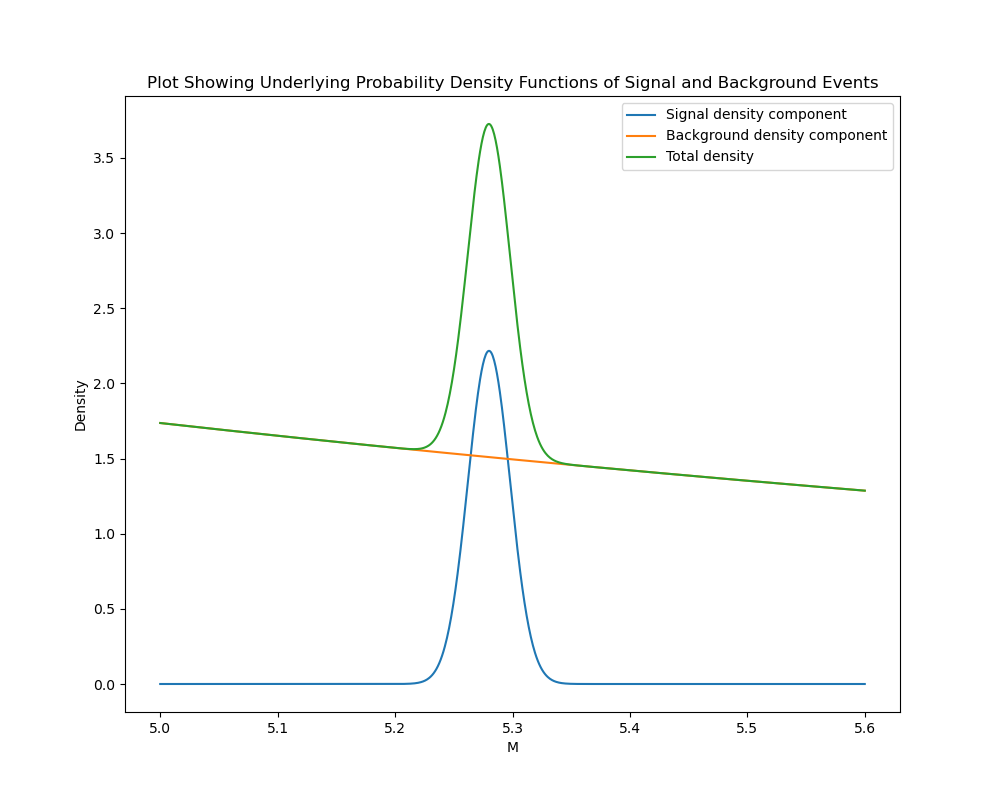
\includegraphics[scale=0.5]{part_d_plot.png}
    \caption{The true underlying distribution of $M$ [generated in Python using Matplotlib].}
    \label{part_d_plot}
\end{figure}

Note that the blue and orange lines, labelled as `density components' are the plots of the probability density functions for $M$ for the signal and background events respectively.
However, to make the plot more intuitive, they have been multiplied by the respective proportion of that type of event in the total population.
This means that technically neither is a probability density function, however their sum is the true mixed density for the population.
The area under either of the component functions limited to an interval smaller than $[5, 5.6]$ is precisely the probability that an event randomly sampled from the population will be of that kind, and lie within said interval.

\subsection*{Part (e)}

In part (e), a large sample is generated from the true distribution, and then the sample is plotted alongside an estimate for the sample's underlying distribution.
Originally, rejection sampling was used to create the sample, but this was found to be quite slow, a problem which was exacerbated in the simulation studies.
Instead, an inverse CDF method was used to generate the sample.
The inverse CDF method involves generating a sample of points uniformly distributed in $[0, 1]$, and then transforming these by the percentage point function (the inverse of the cumulative density function).
This achieves a sample which should theoretically be distributed according to the original probability density function.

This can easily be seen by letting $X$ have distribution $U(0,1)$, and transforming $Y:=F^{-1}(X)$ where $F$ is the cdf of the distribution we wish to sample from.
Then clearly $Y$ has the desired distribution because for any $c\in(-\infty,+\infty)$,

\begin{align*}
    P(Y\in(-\infty, c)) & = P(F^{-1}(X)\in(-\infty, c)) \\
                        & = P(X\in(0, F(c))) & \text{$F$ is monotonic and increasing}\\
                        & = F(c) & \text{$X$ is uniformly distributed}\\
\end{align*}

Hence $Y$ has cdf $F$.

In this case the cumulative distribution for the true density $p$ is intractable, and thus we have to estimate it by sampling it at high granularity using the below block of code.

\begin{lstlisting}[caption=Code block producing array of values for inverse CDF of $p$ (e).]
# Compute CDF values across interval [5.0, 5.6].
cdf_mixed_approx_sb = cdf_norm_expon_mixed(
    input_space, 0.1, 0.5, 5.28, 0.018, 5.0, 5.6
)
quantiles_sb = np.linspace(0.0, 1.0, int(10**GRANULAR))
cdf_mixed_inv_sb_01 = np.zeros(int(10**GRANULAR))
# For each quantile in [0.0, 1.0], find how far into the range [5.0, 5.6] you
# need to go in order for the cdf to equal the quantile.
for quantile_idx, quantile in enumerate(quantiles_sb):
    cdf_mixed_inv_sb_01[quantile_idx] = (10 ** (-GRANULAR)) * np.sum(
        cdf_mixed_approx_sb < quantiles_sb[quantile_idx]
    )
# Transform into the interval [5.0, 5.6].
CDF_MIXED_INV_APPROX_SB = 5.0 + 0.6 * cdf_mixed_inv_sb_01
\end{lstlisting}

We then model the density function of the sample parametrically using a model of the same form as the true distribution $p$.
We estimate the four parameters by using a binned maximum likelihood procedure: first separating the data into 100 bins, and then find maximum likelihood estimates for the parameters based on the binned data.
This is done using the \texttt{iminuit} Python package, which outputs the Hesse error matrix for the estimates as well as the fitted values.

\begin{table}
\centering
\begin{tabular}{| c | c | c |}
    \hline
    Parameter & Estimate & Error Estimate \\
    \hline
    $f$  & 0.0998 & 0.0016 \\
    \hline
    $\lambda$ & 0.505 & 0.019 \\
    \hline
    $\mu$ & 5.28014 & 0.00033 \\
    \hline
    $\sigma$ & 0.01787 & 0.00032 \\
    \hline
\end{tabular}
\caption{Estimates produced by Minuit package.}
\label{tab1}
\end{table}

In Table \ref{tab1} we see the fitted values for the binned maximum likelihood fit for the large sample run in \texttt{solve\_part\_e.py}
We see that the parameter estimates are very close to their true values, with correspondingly low errors.
Table \ref{tab2} gives more information about the errors, displaying the matrix of covariances between the parameter estimates.

\begin{table}
    \centering
    \begin{tabular}{| c | c | c | c | c |}
        \hline
        cov(,) & $f$ & $\lambda$ & $\mu$ & $\sigma$ \\
        \hline
        $f$       & 2.67e-06  & -3.45e-07 & -8.74e-09 &  2.38e-07 \\
        \hline
        $\lambda$ & -3.45e-07 &  0.000373 &  2.81e-07 & -5.07e-08 \\
        \hline
        $\mu$     & -8.74e-09 &  2.81e-07 &  1.08e-07 & -2.39e-09 \\
        \hline
        $\sigma$  & 2.38e-07  & -5.07e-08 & -2.39e-09 &  1.00e-07 \\
        \hline
\end{tabular}
\caption{Matrix of covariances of parameter estimates.}
\label{tab2}
\end{table}

The \texttt{iminuit} package produces this estimate of the covariances by estimating the inverse of the Hessian of the negative log-likelihood function.
The errors in \ref{tab1} are then the square roots of the variances (diagonal entries), that is, estimates of the standard deviations.
These estimates rely on the assumption of a large sample size (which is true in this case) and that the second derivatives of the log-likelihood are relatively constant near the true maximum-likelihood estimate.

The sample is plotted along with its fitted density according to the parameter estimates in Figure \ref{part_d_plot}.
Since the sample is binned, each of the bin counts is treated as a Poisson random variable and hence the errors plotted are the square roots of the bin counts.
Below the main plot, we have a plot of the `pull' values; the residual errors of the bin counts versus the fitted model, divided by the bin errors.
The histogram to the right confirms that these values appear to follow a standard Gaussian distribution (the green line) which indicates that the fitted model is coherent with the sample.
This is further confirmed by the $\chi^2$ value, the sum of the squares of the pulls, which is approximately equal to the number of degrees of freedom, 95, indicating that we have produced a high quality fit, while avoiding modelling the noise present in the data.

\begin{figure}[hbt]
    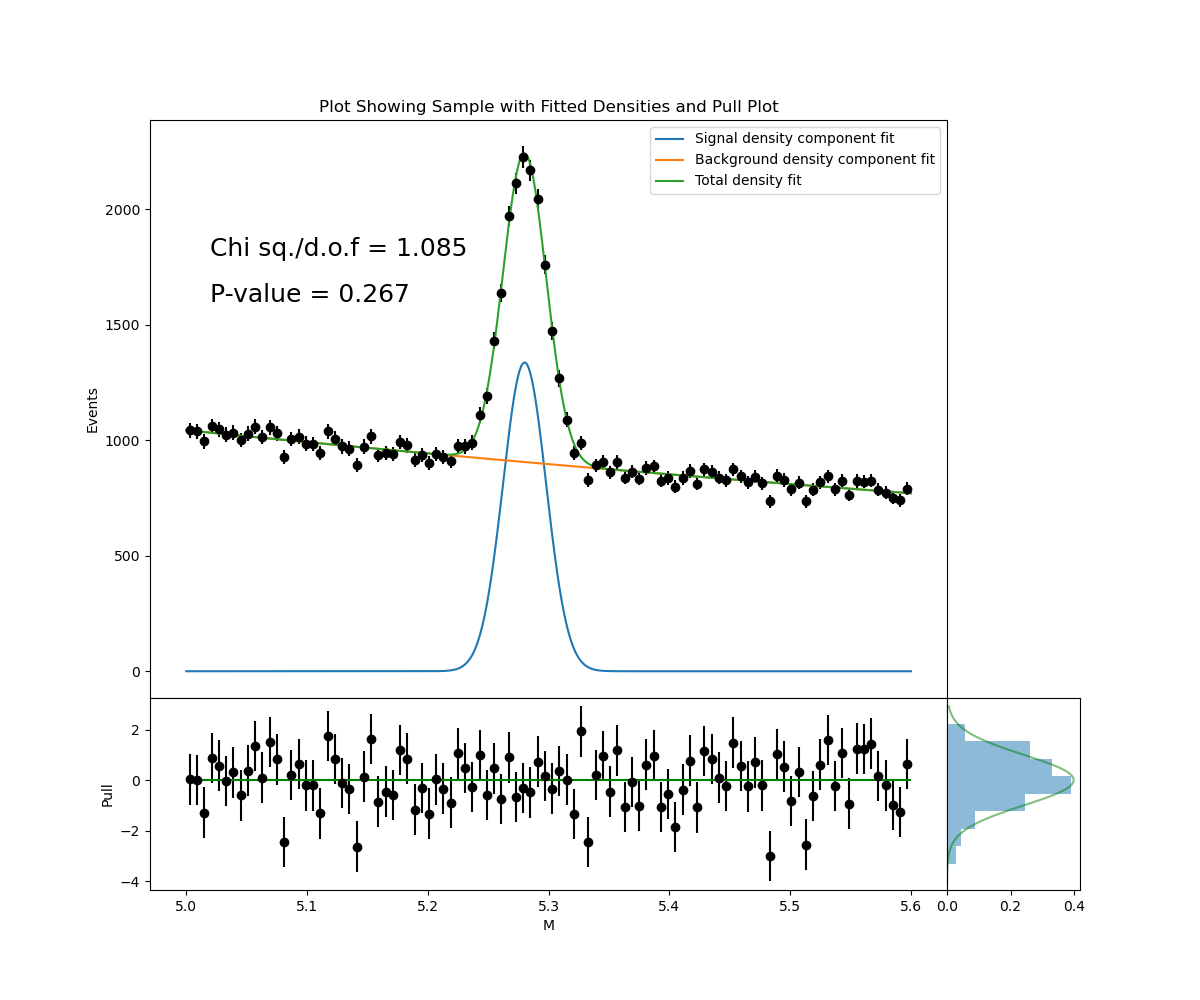
\includegraphics[scale=0.4]{part_e_plot.png}
    \caption{The true underlying distribution of $M$ [generated in Python using Matplotlib].}
    \label{part_e_plot}
\end{figure}

\section*{Section B}

\subsection*{Part (f)}

For this section, the statistical situation involves the null hypothesis $H_0$ that there is no signal present in the data, that is, $f=0$ and the alternative hypothesis $H_1$, that there is at least one signal event, $f\in(0,1]$.
The procedure outline is therefore:
\begin{enumerate}
\label{sim_study_procedure}
    \item Throw a toy, generating a sample of size $N$, $\vec{x}$ from the true distribution.
    \item Use (binned) maximum likelihood estimation to fit the parameters under the $H_0$ model, fixing $f=0$, and obtaining likelihood $L_0(\vec{x})$.
    \item Use ML estimation to fit the parameters under $H_1$ with all parameters floating, to obtain $L_1(\vec{x})$.
    \item Compute the log-likelihood ratio statistic, $T = 2\ln(L_1(\vec{x})/L_0(\vec{x}))$.
    \item Repeat steps 1-4 for a toy generated from the background only distribution.
    \item Repeat steps 1-5 for a high number of toys, $N_{toys}$, to produce distributions of the log-likelihood ratio under $H_0$ and $H_1$.
    \item Use this to compute the discovery rate at a significance level of $2.9\times10^{-7}$.
\end{enumerate}
Steps 2-4 detail the standard statistical procedure that could be used to infer the presence of signal in the given sample, in the realistic setting of an experiment.
However, this relies on having some critical value for the test statistic which we do not have for the statistical model.
Hence steps 5-7 are used to simulate a large number of `toys', datasets independently sampled from the true distribution to estimate the distribution of $T$ under $H_1$, and similarly for the distribution under $H_0$.
The two distributions then enable us to set a critical value $T=T_0$ for discovery according to the specified significance, and to find the resulting statistical power of the test.
In particular, we have
\begin{equation}
\label{eq_significance}
    \text{significance} = P(T>T_0|H_0) = 2.9\times10^{-7}
\end{equation}
\begin{equation}
\label{eq_power}
    \text{power} = P(T>T_0|H_1)
\end{equation}
Equation \ref{eq_significance} fixes the value of $T_0$, above which the test statistic provides evidence for a scientific discovery of at least one signal event, in which case we reject the null hypothesis in favour of the alternate hypothesis.
Equation \ref{eq_power} tells us the statistical power of this test.
In particular, with the desired power, 90\%, the probability of falsely rejecting the alternative hypothesis when it is true is 10\%.
Moreover, since running the simulation we are assuming that the null hypothesis is true, this means that according to our estimated distribution of $T$ under the true distribution, the probability of discovery (of signal) is 90\%, because the $T$ value is above the critical region 90\% of the time.

The discovery rate (in this case the power) is then a function of the sample size $N$ used.
As $N$ increases, the two distributions of $T$ become narrower since the parameter estimate variances decrease.
In turn, the discovery rate at the 5 standard deviation significance level increases since a greater proportion of the true distribution of $T$ lies above the $T_0$.
Hence we run the procedure in \ref{sim_study_procedure} for a range of $N$ until we find the correct value to achieve a 90\% discovery rate.

One of the serious challenges of this simulation study is that $T_0$ is supposed to lie at an extremely high quantile of the distribution of $T$ under the null hypothesis.
Therefore, in order to precisely locate $T_0$, we would ideally produce a sample of $T$ with size $\sim10^8$ in order to ensure that the empirical distribution was based on a sample actually containing some points above the 5 standard deviation quantile.
A lot of time was spent optimising the code in order to achieve this end, but it proved impossible with the given processing and time constraints.

Therefore, the solution was to perform the study with a much smaller number of toys thrown to find $T$, around $\sim10^5$ at most, and then use this to parametrically estimate the true distribution under $H_0$.
Theoretically, Wilk's Theorem \cite{wilks} provides an asymptotic result which ensures that asymptotically as $N$ approaches infinity, twice the negative log-likelihood ratio follows a $\chi^2$ distribution under the null hypothesis, under certain regularity conditions, such as the null hypothesis being simple, the alternate being composite, and the former being a subset of the latter.
Moreover, in this case the degrees of freedom of the $\chi^2$ distribution should be the difference in dimension of the two spaces of parameters for the hypotheses.
In our context some of the regularity conditions have been violated, for instance our null hypothesis $f=0$ lies on the boundary of the parameter space for $H_1$.
However, in many cases such as this one, it has been found that the null hypothesis distribution of $T$ still loosely follows some form of $\chi^2$ distribution, often just with a different degrees of freedom parameter, or a mixture of multiple $\chi^2$ distributions \cite{wilks_exc_1} \cite{wilks_exc_2}.
Therefore we overcome the small number of toys used by fitting a $\chi^2$ model to the sample of $T$ distributed under $H_0$, and using this estimate to find the value of $T_0$ at the required significance level.

In order to find the appropriate trade-off between processing time and accuracy, a preliminary scan of different values of $N$ was performed over a large range of $N$ values, and using a small number of toys, 1000.
This gave an indication of the approximate critical value of $N$.
Then a second simulation study was performed with a much narrower range of sample size values, but using 10000 toys in each case.

These results are recorded in Tables \ref{tab_f_1} and \ref{tab_f_2}.

\begin{table}
    \centering
    \begin{tabular}{| c | c | c | c | c | c |}
        \hline
            N & C. H1 & C. H0 & Valid & T0     & Power    \\
        \hline
           50 & 0.767 & 0.794 & 0.749 & 30.294 & 0.000000 \\
        \hline
          100 & 0.785 & 0.805 & 0.861 & 32.335 & 0.001161 \\
        \hline
          150 & 0.774 & 0.805 & 0.942 & 28.608 & 0.012739 \\
        \hline
          200 & 0.762 & 0.793 & 0.947 & 31.993 & 0.027455 \\
        \hline
          250 & 0.721 & 0.781 & 0.974 & 31.331 & 0.088296 \\
        \hline
          300 & 0.691 & 0.744 & 0.973 & 31.940 & 0.169579 \\
        \hline
          350 & 0.653 & 0.730 & 0.983 & 31.198 & 0.291963 \\
        \hline
          400 & 0.654 & 0.707 & 0.980 & 30.746 & 0.430612 \\
        \hline
          450 & 0.652 & 0.704 & 0.988 & 31.058 & 0.537449 \\
        \hline
          500 & 0.655 & 0.695 & 0.986 & 32.214 & 0.598377 \\
        \hline
          550 & 0.653 & 0.691 & 0.986 & 31.666 & 0.716024 \\
        \hline
          600 & 0.650 & 0.689 & 0.988 & 31.821 & 0.782389 \\
        \hline
          650 & 0.655 & 0.684 & 0.990 & 31.538 & 0.856566 \\
        \hline
          700 & 0.654 & 0.688 & 0.987 & 32.286 & 0.893617 \\
        \hline
          750 & 0.671 & 0.676 & 0.988 & 31.110 & 0.935223 \\
        \hline
          800 & 0.659 & 0.672 & 0.982 & 32.073 & 0.949084 \\
        \hline
          850 & 0.661 & 0.665 & 0.988 & 31.483 & 0.971660 \\
        \hline
          900 & 0.663 & 0.662 & 0.988 & 32.212 & 0.978745 \\
        \hline
          950 & 0.663 & 0.673 & 0.987 & 32.675 & 0.985816 \\
        \hline
         1000 & 0.671 & 0.664 & 0.991 & 31.250 & 0.992936 \\
        \hline
\end{tabular}
\caption{Preliminary simulation study for part (f) using 1000 toys in each case.}
\label{tab_f_1}
\end{table}

In all cases, any time the \texttt{iminuit} package was used to fit the parameter estimates, the estimated errors of these fits, as well as whether or not the software reported that a valid minimum was reached, was recorded.
In the simple cases of fitting the background only model to data sampled from the background only data, and similarly for the mixed model, the coverage of the fitted parameters with respect to the true values was computed, in order to check that all the fits used for the study were of high quality.
If either of the two fits associated to a generated $T$ value were invalid, then that T value was discarded and not used in the study. In all the results the proportion of valid T values (recorded in the `Valid' column) was sufficiently high that the number of toys used was close to the specified amount.
In addition, with the exception of apparent overcoverage in the case of very low sample sizes $N$ in Table \ref{tab_f_1}, we can see that the coverage for the estimates checked when fitting $H_0$ and $H_1$ were close to the expected 68.3\%.

\begin{table}
    \centering
    \begin{tabular}{| c | c | c | c | c | c |}
          N & C. H1   & C. H0    & Valid   & T0       & Power    \\
        700 & 0.654   & 0.685    & 0.985   & 31.669   & 0.893198 \\
        705 & 0.655   & 0.687    & 0.986   & 31.779   & 0.897272 \\
        710 & 0.660   & 0.683    & 0.985   & 31.578   & 0.904182 \\
        715 & 0.659   & 0.684    & 0.987   & 31.617   & 0.906548 \\
        720 & 0.655   & 0.680    & 0.985   & 31.788   & 0.909063 \\
        725 & 0.658   & 0.682    & 0.986   & 31.799   & 0.912854 \\
        730 & 0.661   & 0.682    & 0.986   & 31.679   & 0.916819 \\
        735 & 0.660   & 0.684    & 0.986   & 31.888   & 0.916607 \\
        740 & 0.661   & 0.684    & 0.988   & 31.746   & 0.921785 \\
        745 & 0.660   & 0.684    & 0.986   & 32.016   & 0.922203 \\
        750 & 0.663   & 0.685    & 0.984   & 31.744   & 0.927548 \\
    \end{tabular}
\caption{Second simulation study for part (f) using 10000 toys in each case.}
\label{tab_f_2}
\end{table}

In Table \ref{tab_f_2} we see that the critical value to achieve 90\% power is somewhere in the range $N=705$ and $N=710$; interpolating linearly we estimate that 707 data points are required for a 90(.0036)\% discovery rate.

\bibliography{Biblio}

\end{document}
